%!TEX root = ../main.tex
\section{Joint Development}
\label{sec:joint_development}
In creating a pendulum the mounting point must be able to rotate freely about the mounting axis.
To achieve this a joint must be designed which can accomodate this motion.
Throughout this section the analysis, design and implementation of this joint is explored.

%!TEX root = ../main.tex
\subsection{Analysis} % (fold)
\label{sub:analysis}

In the system analysis a number of requirements were found relating to the design of the joints.
These requirements contain both mechanical and electrical aspects.
The authors' main focus is on power and embedded design and as such the design of the mechanics of the system is limited in comparison to the electrical design.
The mechanical design was developed with advice from mechanical engineer at SDU: Jørgen Maagaard.

\subsubsection{Mechanics} % (fold)
\label{ssub:mechanics}
The mechanical design consists of two parts, the joint and the rod connecting two joints.
This project seeks to create a two-joint pendulum but the project owner has set a few additional requirements to allow for more diverse control tasks in future projects:
\begin{itemize}
	\item It should be possible to mount $n$ joints in series on the pendulum assembly.
	\item The distance between the joints should be modular.
\end{itemize}
In addition to these two requirements:
\begin{itemize}
	\item The pendulum assembly should be rigid and allow only movement in the X-Y plane so that it cannot collide with itself.
\end{itemize}

The first two requirements would benefit from a modular design, allowing the rod to be dismounted from the joint so that only the rod would require replacement, should the user wish to add joints or vary the distance between joints.
This is somewhat in conflict with the last requirement, which would benefit from each joint-rod-joint assembly to be one solid piece of material.
Since such an assembly would be rather expensive to manufacture and would require a new assembly for each desired configuration, a modular design is preferred.
\\~\\
The joint should be capable of unrestricted rotation.
This rotation should be as close to frictionless as possible and so a low friction coupling should be used between the two parts of the joint.
As will be discussed in section \ref{ssub:encoder} some form of encoder is required in the joint.
This encoder requires both power and signal wiring.
Two solutions were considered to solve this problem
\begin{itemize}
  	\item \textbf{Slip Ring:} A slip ring allows wiring to pass through a freely rotating joint.
  	They are available in versions of various sizes with up to 72 wires, allowing for several series joints before being limited by wire capacity.
  	Clearly, more wires results in a longer slip ring, imposing additional requirements to the thickness of the joint to accomodate for the slip ring.
  	The authors were in contact with Rotary Systems and Moog, both industry suppliers of slip rings and similar products.
  	It was clear that the price of these components was well beyond what is reasonable for this project.
  	\item \textbf{Wireless:} Several wireless solutions exist which could be employed in this situation.
  	Using a wireless approach means that all computation and handling of signals must be done on the joint before transmitting to the main controller.
  	This means that a more complex PCB must be designed and a battery installed to power the PCB.
  	While this solution does add electrical complexity it is practically free in comparison to the slip ring and allows for a much slimmer joint design.
  	This is the solution chosen for the joint design.
\end{itemize}
~\\
As discussed in the State of the Art analysis the pendulum assembly is viewed as a collection of point-masses connected with massless rods.
In order to more accurately uphold this assumption the material of the rods should be significantly lighter than the material of the joints while still maintaining sufficient rigidity.
In general three materials are easily available to the authors for manufacturing:
\begin{itemize}
	\item \textbf{Metal:} While this is a somewhat vague description that spans a vast number of materials, metals are generally significantly heavier than the following materials.
	Using metals requires manufacturing techniques and equipment which the authors do not have access to but the SDU Workshop can be hired to manufacture a design.
	The precision of metal-working is well into the sub-millimeter range.
	\item \textbf{3D Print:} This method of manufacturing is easily accessible and can be done for free (to the project). 
	It also allows for creating shapes that are otherwise difficult to manufacture in metals.
	3D printing at SDU is done in different types of plastics, neither of which is as stiff as would be desired for the pendulum assembly.
	Additionally, the encoder chosen in the following section sets strict requirements on the placement of the two parts of the encoder (This is discussed in more detail below) and the 3D printers at SDU are known to have problems accurately representing features in the sub-millimeter range.
	\item \textbf{Carbon:} This material is considered only for the rod as it was suggested as a light material with significant rigidity.
	Carbon tubes have been used previously at SDU Vikings, the SDU Formula Student racing team, as part of the suspension assembly.
\end{itemize}
Given the above materials the joint is to be made of metal while a carbon tube will be procured for the rod.
The design should be made such that the SDU Workshop can manufacture the joints and any appertaining components.
% subsubsection mechanics (end)

\subsubsection{Encoder} % (fold)
\label{ssub:encoder}
Each joint should implement an encoder to enable tracking the angular position of the joint.
The resolution of each joint should be sufficient to allow for proper control.
From the State of the Art analysis it was found that a resolution of 8192 ticks per revolution was succesfully used in two systems \cite{doubleinvertpendulum} \cite{tripleinvertpendulum}.
In addition to resolution, ease of manufacture and design is also an important aspect.
One encoder in particular was recommended to the authors; the Rolin Rotary Magnetic Encoders.
This is a series of encoders which, as the name suggests, utilises magnetic fields in order to determine the angular position of the encoder.
They consist of a magnetic ring with a number of poles and a PCB sensor.
The magnetic ring is available in different sizes with different number of poles which, along with the type of PCB sensor decides the resolution of the encoder.
The specific encoder configuration used in this project, the \texttt{RL2IC} \cite{RLC2IC}, allows for 7200 CPR or one count per 0.05$^\circ$.
The encoder is incremental with an \texttt{A}, \texttt{B} and \texttt{Z} channel where \texttt{A} and \texttt{B} are 90$^\circ$ out of phase and \texttt{Z} is a unique reference mark.
Using the reference mark it is possible to maintain absolute knowledge of the angular position of the joint after the initial encounter with the reference mark.
This is only possible assuming that there is no drift or slippage in the system, a reasonable assumption considering the mechanical setup.
Communication with the encoder is done using the RS422 standard.
This standard describes a method of transmitting digital signals using differential signals and requires specialised hardware to translate between ordinary digital signals and RS422.

% subsubsection encoder (end)
\subsubsection{Electronics} % (fold)
\label{ssub:electronics}
As per the initial requirements listed in this section each joint should be able to track the position of the joint and communicate this information wirelessly to the main controller board.
In order to accomplish this task some form of microcontroller is required along with the power delivery and the RS422 receiver mentioned previously.
The microcontroller must fulfill the following requirements:
\begin{itemize}
 	\item Must have support for three interrupt pins, one for each channel of the encoder.
 	\item Must have an SPI interface to maintain communication with the\\ \texttt{nRFM}.
 	\item Must have non-volatile memory to store the program through power cycling the board.
\end{itemize}
The \texttt{ATtiny84} \cite{attiny84} fulfills these requirements and provides sufficient I/O pins for the design.
The design of the PCB and the layout in general should accomodate the joint design.
By minimizing the height of the PCB design, the joint can be made thinner, reducing the stress on the pendulum assembly along the Z-axis.
It should also be noted that any connectors should be placed with the expectation that the border of the PCB is not accessible during normal operation.
\\~\\
Since the PCB is powered from a battery the design should be optimized to be reasonably power efficient.
As is explained in the next section, the design has a 3.3V rail and a 5V rail.
Generally microcontrollers become more power efficient at lower voltages and as such the \texttt{ATtiny} will be driven from the 3.3V rail.
The authors have immediate access to an AVR programmer which uses 5V signals for the programming.
The design should be made to accept this voltage when programming.
This can be done using level-shifting between the two voltage levels.
\\~\\
It was chosen to add an LED to the design for debugging purposes.
Clearly, an LED does require some power and should not be used during normal operation.
\paragraph{Power Delivery}~\\ % (fold)
\label{par:power_delivery}
The required voltage rails on the joint board are dictated by the RF module and the encoder.
The former requires 3.3V and the latter 5V.
Since the joints are to be wireless it is necessary to power them from a battery.
To avoid added complexity there will be no charging circuitry and charging the battery should be done externally to the joint.
The battery of the joint should last for as long as is possible while still fitting within the enclosure.
This requirement essentially narrows the battery choices to LiPo cells as these generally have the highest energy density of the commercially avaiable battery types.
1S LiPo cells are rated at 3.7V and so some form of convertion is required to reach both the 5V and 3.3V rails.
In order to correctly dimension the converters it is necessary to determine the power draw from each rail:
\begin{itemize}
 	\item \textbf{3.3V:} This rail powers the \texttt{nRFM} which has a maximum supply current of 12.3mA \cite{NFR24L01} as well as the \texttt{ATTiny}.
 	According to the datasheet of the \texttt{ATtiny} it uses approximately 3.6mA at 3.3V when run at 8MHz.   
 	This yields a total of 15.9mA at 3.3V or 52.5mW.
 	Additional digital circuitry placed on this rail is considered negligible in the power budget.
 	\item \textbf{5V:} This rail powers the encoder with a maximum supply current of 30mA \cite{RLC2IC} as well as the RS422 receiver which has a supply current of 52mA \cite{rs422rec}.
 	This yields a total of 82mA at 5V or 410mW.
 	Additional digital circuitry placed on this rail is considered negligible in the power budget.
\end{itemize}
For a battery to have sufficient capacity to power the joint for a full workday, estimated at 10 hours, it should have at least $\approx4600$mWh.
This is infeasible in the required dimensions and a battery should be procured which can provide the most run time given the space available.
\\~\\
The voltage rails should be designed with sufficient overhead.
Additionally, the accuracy of each rail is determined from the supply requirements set by the datasheet of the components used in the datasheet.
The two rails should be specced as follows:
One rail capable of delivering 200mA at 5V$\pm$0.2V.
One rail capable of delivering 100mA at 3.3V$\pm$0.2V.
% paragraph power_delivery (end)
% subsubsection electronics (end)

\subsection{Requirement Specification}
\label{subs:joint_requirements}
The requirements specified below are tested and verified in section \ref{sub:verification_joint_board_}.
\paragraph{Functional:}
\begin{enumerate}[resume]
	\item Pendulum assembly should allow movement only in the X-Y plane. 
	\label{enum:pendulum_should_only_x_y}
	\item Voltage rails for the components in the circuit.
	\label{enum:joint_voltage_rails}
	\begin{itemize}
		\item At least 100mA at 3.3V$\pm$0.2V.
		\item At least 200mA at 5V$\pm$0.2V.
	\end{itemize}
	\item Joint should be able to rotate freely about the mounting axis.
	\label{enum:rotate_freely_joint}
	\item The \texttt{nRFM} should be included for communication.
	\label{enum:joint_include_nrf}
	\item the RS422 interface of the \texttt{RL2IC} encoder should be correctly interfaced.
	\label{enum:interface_rs422_enc}
	\item The design should allow programming of the \texttt{ATtiny} using 5V SPI.
	\label{enum:program_5v_spi}
	\item An LED should be employed for debugging purposes.
	\label{enum:led_debugging_joint}
\end{enumerate}

\paragraph{Design:}
\begin{enumerate}[resume]
	\item Weight of rods should be minimized to uphold the point mass assumption.
	\label{enum:design_req1}
	\item Joints should be designed in a modular fashion such that $n$ joints can be mounted in series.
	\label{enum:design_req2}
	\item Distance between joints should be adjustable.
	\label{enum:design_req3}
	\item Friction in the joint should be minimized.
	\label{enum:design_req4}
	\item Design of the joint should employ mounting solutions for:
	\label{enum:design_req5}
	\begin{itemize}
		\item Joint board.
		\item Encoder.
		\item Battery. 
	\end{itemize}
	\item The design of the joint should be done so that it can be manufactured by the SDU workshop.
	\label{enum:design_req6}
	\item The PCB should be designed with the enclosure in mind.
	\label{enum:design_req7}
	\begin{itemize}
		\item Height of components and general design should be minimized.
		\item Placement of connectors should accomodate the enclosure.
		\item Shape of the PCB should allow for easy mounting of the PCB and other components.
	\end{itemize}
	\item The PCB layout should be reviewed according to the developed strategy.
	\label{enum:design_req8}
	\begin{itemize}
		\item Documentation.
		\item General inspection.
		\item Datasheet and report comparison.
		\item Footprint inspection.
		\item Peer-review.
	\end{itemize}
	\item A Battery should be sourced which conforms with the following requirements:
	\label{enum:design_req9}
	\begin{itemize}
		\item Battery should provide power for the joint for as long as possible.
		\item Battery should fit within the dimensions dictated by the enclosure.
	\end{itemize}
	\item Overall power consumption of the design should be minimized.
	\label{enum:overall_joint_power}
\end{enumerate}
% subsection analysis (end)
%!TEX root = ../main.tex
\subsection{Joint Design} % (fold)
\label{sub:joint_design}
The design of the pendulum assembly is, as in the analysis, split into an electrical design and a mechanical design.

\thomas{Proper introduction required}

\subsubsection{Mechanical Design} % (fold)
\label{ssub:mechanical_design}
The mechanical design consists mainly of 3D modelling using Autodesk Inventor.
The entire design is shown in figure \ref{fig:mechdesign} and is comprised of three parts:
\paragraph{Magnet Side:} % (fold)
\label{par:magnet_side}
is shown in figure \ref{sfig:magnetside}. 
This part has a shallow groove milled for the magnetic disc of the encoder to fit into.
The centre of the part is milled out to allow for two low-friction ball bearings to be press-fit into.
% paragraph magnet_side (end)
\paragraph{Reader Side:} % (fold)
\label{par:reader_side}
is shown in figures \ref{sfig:readside} and \ref{sfig:readside_2}.
The visible sides of \ref{sfig:magnetside} and \ref{sfig:readside} are designed to mate.
A cutout is made in \ref{sfig:readside} which is positioned such that it can be placed accurately above the magnetic disc.
The placement of the reader head by pressing it against a feeler gauge blade positioned between it and the magnetic disc before securing it using two bolts.
This ensures that the reader head is placed parallel with the disc and at the correct distance.
The axle is milled as part of \ref{sfig:readside}.
The manufactured version has a bore in the axle to accomodate a bolt which tightens the part to the bearings.
On the other side of the part, \ref{sfig:readside_2}, most of the material has been bored away to allow for mounting the joint board as shown in the figure.
A lip has been left on top of the part to allow for mounting a lid.

\paragraph{Joint Mount:} % (fold)
\label{par:joint_mount}
is shown in \ref{sfig:jointmount}.
This component was made to mate the joint with the joint rod.
A hole pattern is added to this part as well as the other two which is used to mount \ref{sfig:jointmount} to \ref{sfig:readside} and \ref{sfig:magnetside}.
On the top of the part a hole is made to accomodate the joint rod.
This part is 3D printed since the shape is somewhat complex and would require access to a CNC machine to mill of metal.
Additionally, making the part from metal would increase its weight significantly, potentially risking the point-mass assumption.
\\~\\
These three parts are connected into the pendulum assembly using carbon tubes as shown in \ref{sfig:pendulumassembly}.
Two parts are present on this design which were not described previously.
The final disc, known as the dummy disc, is essentially just a solid piece of aluminium used to add some weight to the end of the pendulum assembly.
The second part is a plate which the first joint is mounted on which is to be mounted on the cart.

\thomas{fix figure text below}
\begin{figure}[H]
	\begin{minipage}{.45\linewidth}
		\begin{subfigure}[b]{\linewidth}
			\centering
			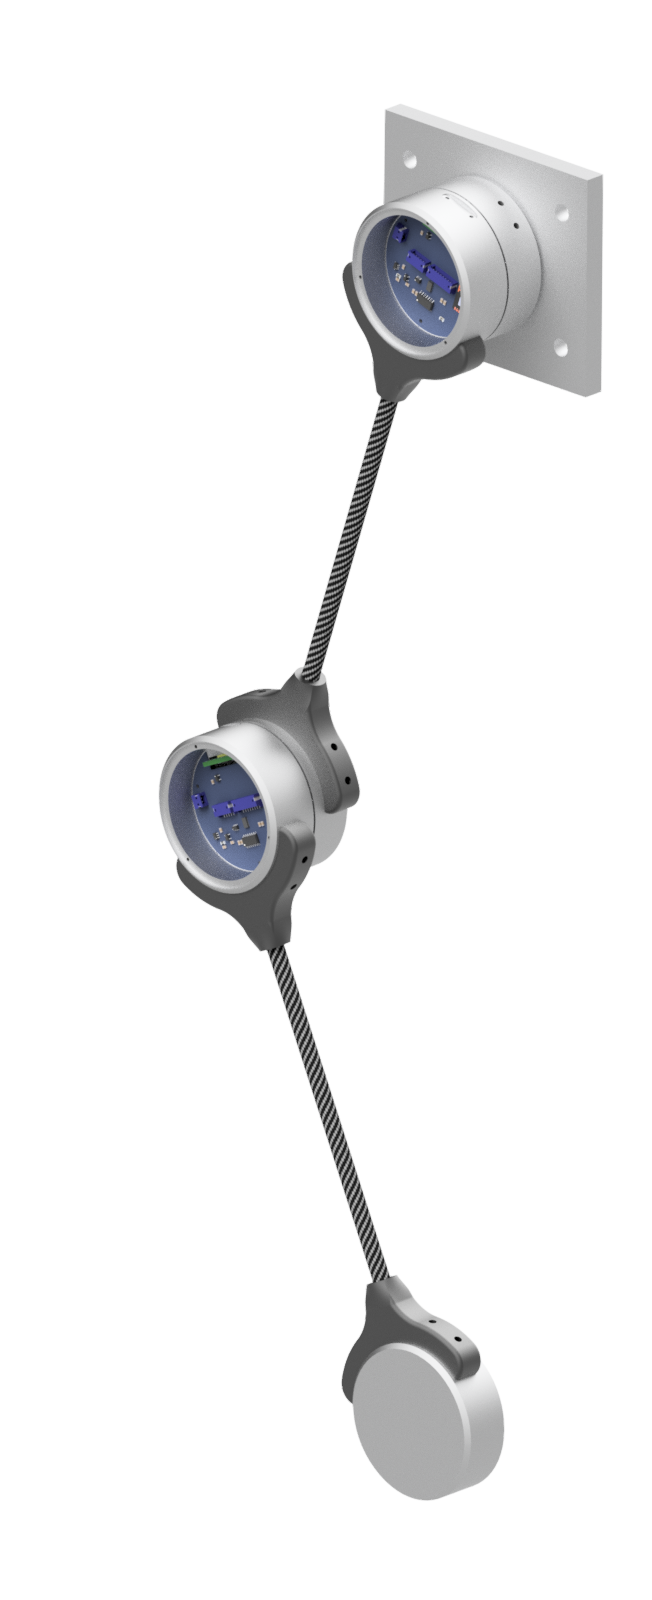
\includegraphics[width=.85\linewidth]{graphics/pendulum_assembly}
			\caption{This is a line of text}
			\label{sfig:pendulumassembly}
		\end{subfigure}\\
		\begin{subfigure}[b]{\linewidth}
			\centering
			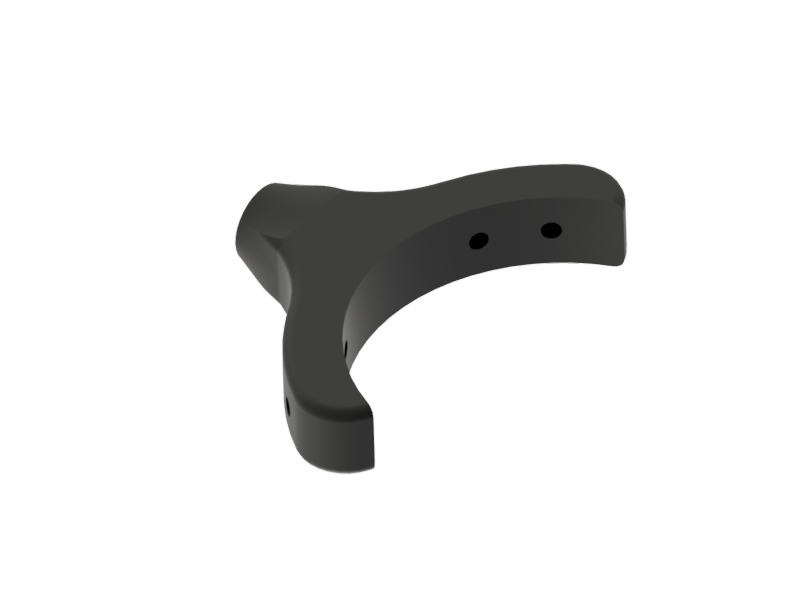
\includegraphics[width=\linewidth]{graphics/joint_mount}
			\caption{No one ever reads me... and some more text to fill out the caption}
			\label{sfig:jointmount}
		\end{subfigure}	
	\end{minipage}
	\begin{minipage}{.4\linewidth}
		\begin{subfigure}[t]{\linewidth}
			\centering
			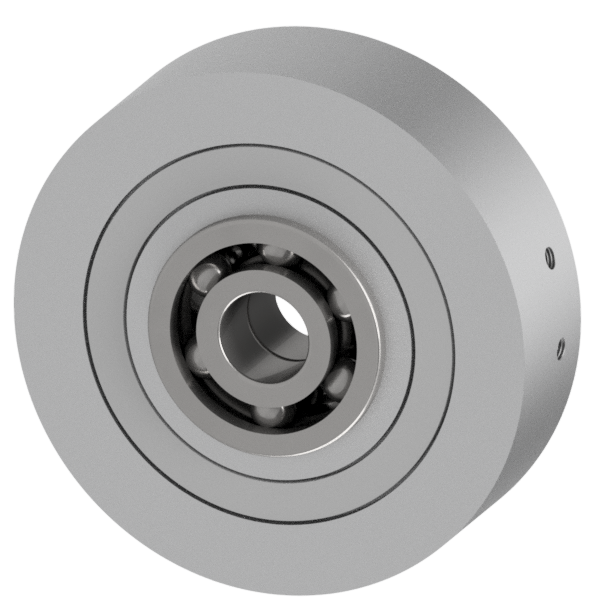
\includegraphics[width=\linewidth]{graphics/joint_mag_assembly}
			\caption{So is this..}
			\label{sfig:magnetside}
		\end{subfigure}\\
		\begin{subfigure}[b]{\linewidth}
			\centering
			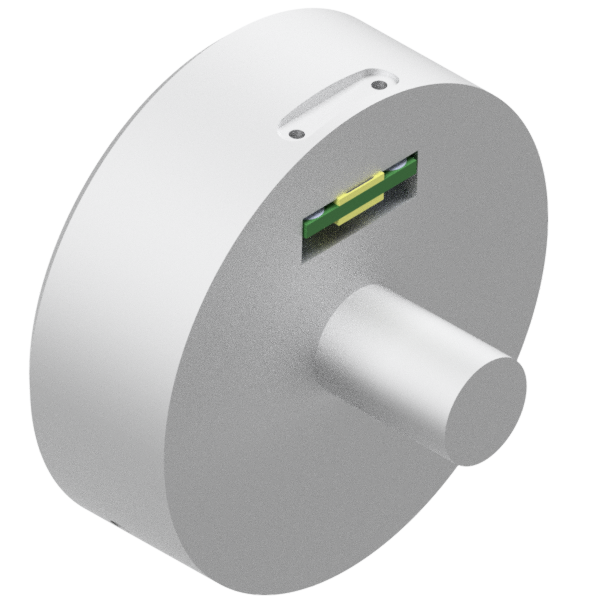
\includegraphics[width=\linewidth]{graphics/joint_read_side}
			\caption{And this!}
			\label{sfig:readside}
		\end{subfigure}\\
		\begin{subfigure}[b]{\linewidth}
			\centering
			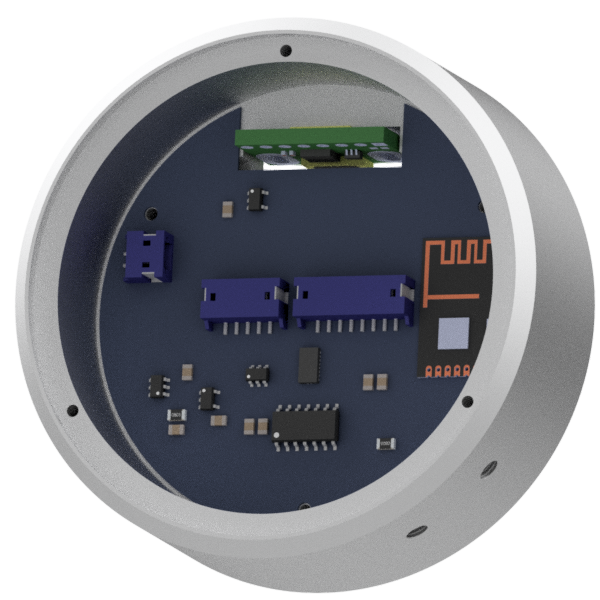
\includegraphics[width=\linewidth]{graphics/joint_read_side_2}
			\caption{Me too! this needs some more text as well. So here it is}
			\label{sfig:readside_2}
		\end{subfigure}
	\end{minipage}
	\caption{Me be Big-Momma Text!}
	\label{fig:mechdesign}
\end{figure}

\subsubsection{RS422}
The \texttt{RL2IC} uses the RS422 standard for its output.
This means that each \texttt{A}, \texttt{B} or \texttt{Z} channel consists of a two wire differential signal.
A line receiver is needed in order to translate the RS422 signals to logic inputs that the ATtiny84 can read.
The \texttt{DS26LS32CM} is a quad differential line receiver that complies with the RS422 standard.  
When using RS422 there are different termination methods, with no termination being the simplest.
The RS422 Standard Overview \cite{rs422_texas} describes that signal integrity is maintained in a setup of \approx 30m wires carrying data at a signal rate of 200kbps without termination.
The intended setup on the joint board requires wires no longer than 5cm.
The maximum expected data rate can be calculated using the maximum expected angular velocity of the joint of 20Hz and the edges on one channel per revolution.
\begin{equation}
Datarate_{max}	= 20 \cdot 3600 = 72kbps
\end{equation}
This datarate is clearly below the 200kbps and it was therefore decided to use no line termination, which also has the advantage that a minimum amount of current is needed from the \texttt{RL2IC}.


\subsubsection{5V}
As described in the requirements in section \ref{subs:joint_requirements}, a 5V rail is needed on the joint board.
Generating the 5V rail can be done by boosting the battery voltage up to 5V, as the battery voltage will always be lower than 5V.
The boost regulator \texttt{SP6641B} \cite{sp6641b} has an input range of 0.9V to 4.5V and a fixed output of 5V.
The circuitry used in this project will be based on the reference design shown in the datasheet, with the one difference that the \texttt{SHDN} (shutdown) pin has been pulled permanently high.

\subsubsection{3.3V}
A 3.3V rail is needed according to the requirement specification.
The task of generating the 3.3V rail is somewhat complicated since the battery voltage of a typical Li-Ion battery varies from 4.2V down to 3.0V.
Three different solutions appeared after an initial analysis of the task:

\begin{itemize}
	\item Buck converter
	\item Buck-Boost converter
	\item Linear regulator
\end{itemize}

The qualities and drawbacks of the three solutions are presented here.

\paragraph{Buck Converter:}
The voltage from the battery can be converted to 3.3V using a Buck converter.
A Buck converter is relatively simple and circuitry can easily be designed for the task.
It is only able to supply an output voltage that is lower than the input voltage.
Which means that when the battery voltage is lower than 3.3V the converter will stop producing a stable 3.3V output.
This means that a portion of the battery capacity cannot be used.
The \texttt{TPS62220} is a Buck regulator and generally has good specifications for this task. 
With an input voltage of 3.7V and an output voltage of 3.3V it has an efficiency of approximately 95\% with an output current in the range of 1mA to 20mA \cite{TPS6222}.
The minimum drop out voltage of the \texttt{TPS62220} is low, because it has a 100\% duty cycle mode.
In this mode, the the drop out voltage is purely defined by the \texttt{ON} resistance of the internal switch, the DC resistance of the external inductor and the output current.

The drop out voltage can be calculated using equation \ref{eq:drop_v_tps62}, \cite{TPS6222}.
\begin{equation}
	V_{drop} = I_{O} \cdot (R_{DS(on),max}+R_I)
	\label{eq:drop_v_tps62}
\end{equation}

\begin{equation}
	V_{drop} = 0.02 \cdot (0.67+0.09) = 15 [mV]
	\label{eq:drop_v_tps62_2}
\end{equation}

Where $I_O$ is the output current, $R_{DS(on),max}$ is the \texttt{ON} resistance of the internal switch and $R_I$ is the DC resistance of the external inductor.
The inductor resistance used is found in the \texttt{LQH55D} SMD inductor \cite{LQH55D}.
\mikkel{Update to new inductor and change equations above}
This means that it can supply 3.3V output when the input voltage is 3.315V or greater



\paragraph{Buck-Boost Converter:}
The motivation for using a Buck-Boost converter is to allow for full utilization of the battery capacity.
This requires that the converter can make a seamless transition between the stepping up and stepping down of the input voltage. 
\texttt{TPS6300} is a Buck-Boost regulator that has these features.
The external circuitry is simple, but the drawback of this regulator and converter is the efficiency of it.
With an input voltage of 3.7V and an output voltage of 3.3V it has an efficiency of approximately 75\% with an output current in the range of 1mA to 20mA \cite{TPS6300}.

\paragraph{Linear Regulator:}
A linear regulator is a component that can regulate the output voltage by varying an internal resistance.
Linear regulators have a drop voltage that limit the output voltage. 
The \texttt{LD3985} has an ultra low drop voltage of 20mV at 50mA output current \cite{LD3985}.

Therefore the efficiency is proportional to ratio between the output and input voltage and can be estimated using equation \ref{eq:eff_lin} \cite{ap_note_140}.

\begin{equation}
	\eta \simeq \frac{V_{out}}{V_{in}}
	\label{eq:eff_lin}
\end{equation}

The voltage of a Li-Ion battery varies from 4.2 to 3.0V, but the nominal voltage is 3.7V and this will be used as an estimate of the mean voltage of the battery.
Using this the mean efficiency can be estimated as shown in equation \ref{eq:eff_lin_val}.

\begin{equation}
	\eta \simeq \frac{3.3}{3.7} = 0.89 = 89\%
	\label{eq:eff_lin_val}
\end{equation}


\paragraph{Comparison}
The most important parameters of the three solutions discussed are shown in table \ref{tab:vol_gen_joint}.

\begin{table}[h]
	\centering
	\begin{tabular}{l|c|c|c}
		  				&	Buck 	& Buck-Boost 	& Linear\\
		 \hline
		 Efficiency  	&  95\% 	& 75\%			&89\%		\\
		 Drop out [mV]		&15  	& N/A		&20		\\
	\end{tabular}
	\caption[Parameters of voltage generation solutions.]{Parameters of the three solutions using a Buck converter, Buck-Boost converter or a linear regulator. The efficiency shown is estimated with an input voltage of 3.7V, an output voltage of 3.3V and an output current in the range of 1mA to 20mA. The drop out voltage is estimated with an output current of 20mA (Buck) and 50mA (linear regulator).}
	\label{tab:vol_gen_joint}
\end{table}

The Buck converter solution has the highest efficiency and is therefore the natural choice.
As already discussed the disadvantage of using a Buck converter is that the full battery capacity cannot be utilized.
A discharge test should be conducted to determine the amount of capacity that cannot be utilized.


\paragraph{Battery Discharge}
At the time of writing, the chosen battery has not yet been procured and the test will therefore be conducted on a similar battery instead.
The battery under test is a 850 mAH Li-Ion battery with the dimensions 49mm X 29mm X 6mm.
It should be noted that both the capacity and physical dimensions are similar to the chosen battery.
The discharge curve of the two batteries will not be identical, but will be sufficiently close to to allow for deciding which solution should be used.
The test was conducted by connecting the battery to an electrical load programmed to discharge with a constant power of 0.3 Watt, while measuring the battery voltage.
The measured discharge curve is shown in figure \ref{fig:bat_discharge}.

\begin{figure}[h]
	\centering
	%%% This file was created by matlab2tikz.
%
%The latest updates can be retrieved from
%  http://www.mathworks.com/matlabcentral/fileexchange/22022-matlab2tikz-matlab2tikz
%where you can also make suggestions and rate matlab2tikz.
%
\definecolor{mycolor1}{rgb}{0.00000,0.44700,0.74100}%
%
\begin{tikzpicture}

\begin{axis}[%
width=4.521in,
height=3.566in,
at={(0.758in,0.481in)},
scale only axis,
xmin=0,
xmax=450,
xlabel style={font=\color{white!15!black}},
xlabel={Time [Min]},
ymin=2.5,
ymax=4.5,
ytick={2.5,   3, 3.5,   4, 4.5},
ylabel style={font=\color{white!15!black}},
ylabel={Voltage [V]},
axis background/.style={fill=white},
title style={font=\bfseries},
title={Discharge Curve of Li-Ion Battery}
]
\addplot [color=mycolor1, forget plot]
  table[row sep=crcr]{%
0	4.072\\
10	4.02699999999999\\
20	4.00799999999998\\
40	3.95999999999998\\
50	3.92200000000003\\
60	3.89499999999998\\
70	3.87900000000002\\
80	3.85500000000002\\
90	3.84300000000002\\
100	3.81799999999998\\
110	3.79700000000003\\
120	3.78899999999999\\
130	3.77699999999999\\
140	3.767\\
150	3.75299999999999\\
160	3.76100000000002\\
170	3.75999999999999\\
180	3.74000000000001\\
190	3.72500000000002\\
200	3.71300000000002\\
210	3.714\\
220	3.69999999999999\\
230	3.71100000000001\\
240	3.71199999999999\\
250	3.69999999999999\\
260	3.69299999999998\\
270	3.69099999999997\\
280	3.69799999999998\\
290	3.69099999999997\\
300	3.68099999999998\\
310	3.673\\
320	3.65699999999998\\
330	3.64499999999998\\
340	3.63499999999999\\
350	3.62299999999999\\
360	3.60700000000003\\
370	3.61399999999998\\
380	3.596\\
390	3.56799999999998\\
400	3.505\\
410	3.36099999999999\\
414.551694551695	2.30000000000001\\
};
\addplot [color=red, dashed, forget plot]
  table[row sep=crcr]{%
0	3.30000000000001\\
450	3.30000000000001\\
};
\end{axis}
\end{tikzpicture}%
	\caption[Discharge curve of Li-Ion battery.]{Voltages measured across a 850 mAH Li-Ion battery while discharging using an electrical load programmed to 0.3 Watt. Horizontal red line represents the 3.3V level.}
	\label{fig:bat_discharge}
\end{figure}

It can be observed that the battery voltage only drops below 3.3V for a very short time before the battery is completely discharged.

\paragraph{Conclusion}
The Buck converter solution has the highest efficiency and has a lower drop out voltage than the linear regulator solution.
The disadvantage of using a Buck converter is that the full battery capacity cannot be utilized, but a test showed that almost all of the capacity can be used.
Therefore it was chosen to use a Buck converter with the \texttt{TPS62220} regulator. 
The Buck converter circuit used is based on the recommendations in the datasheet of the \texttt{TPS62220}.
The circuit is shown in figure \ref{fig:tps62220_circuit}.

\begin{figure}[h]
	\centering
    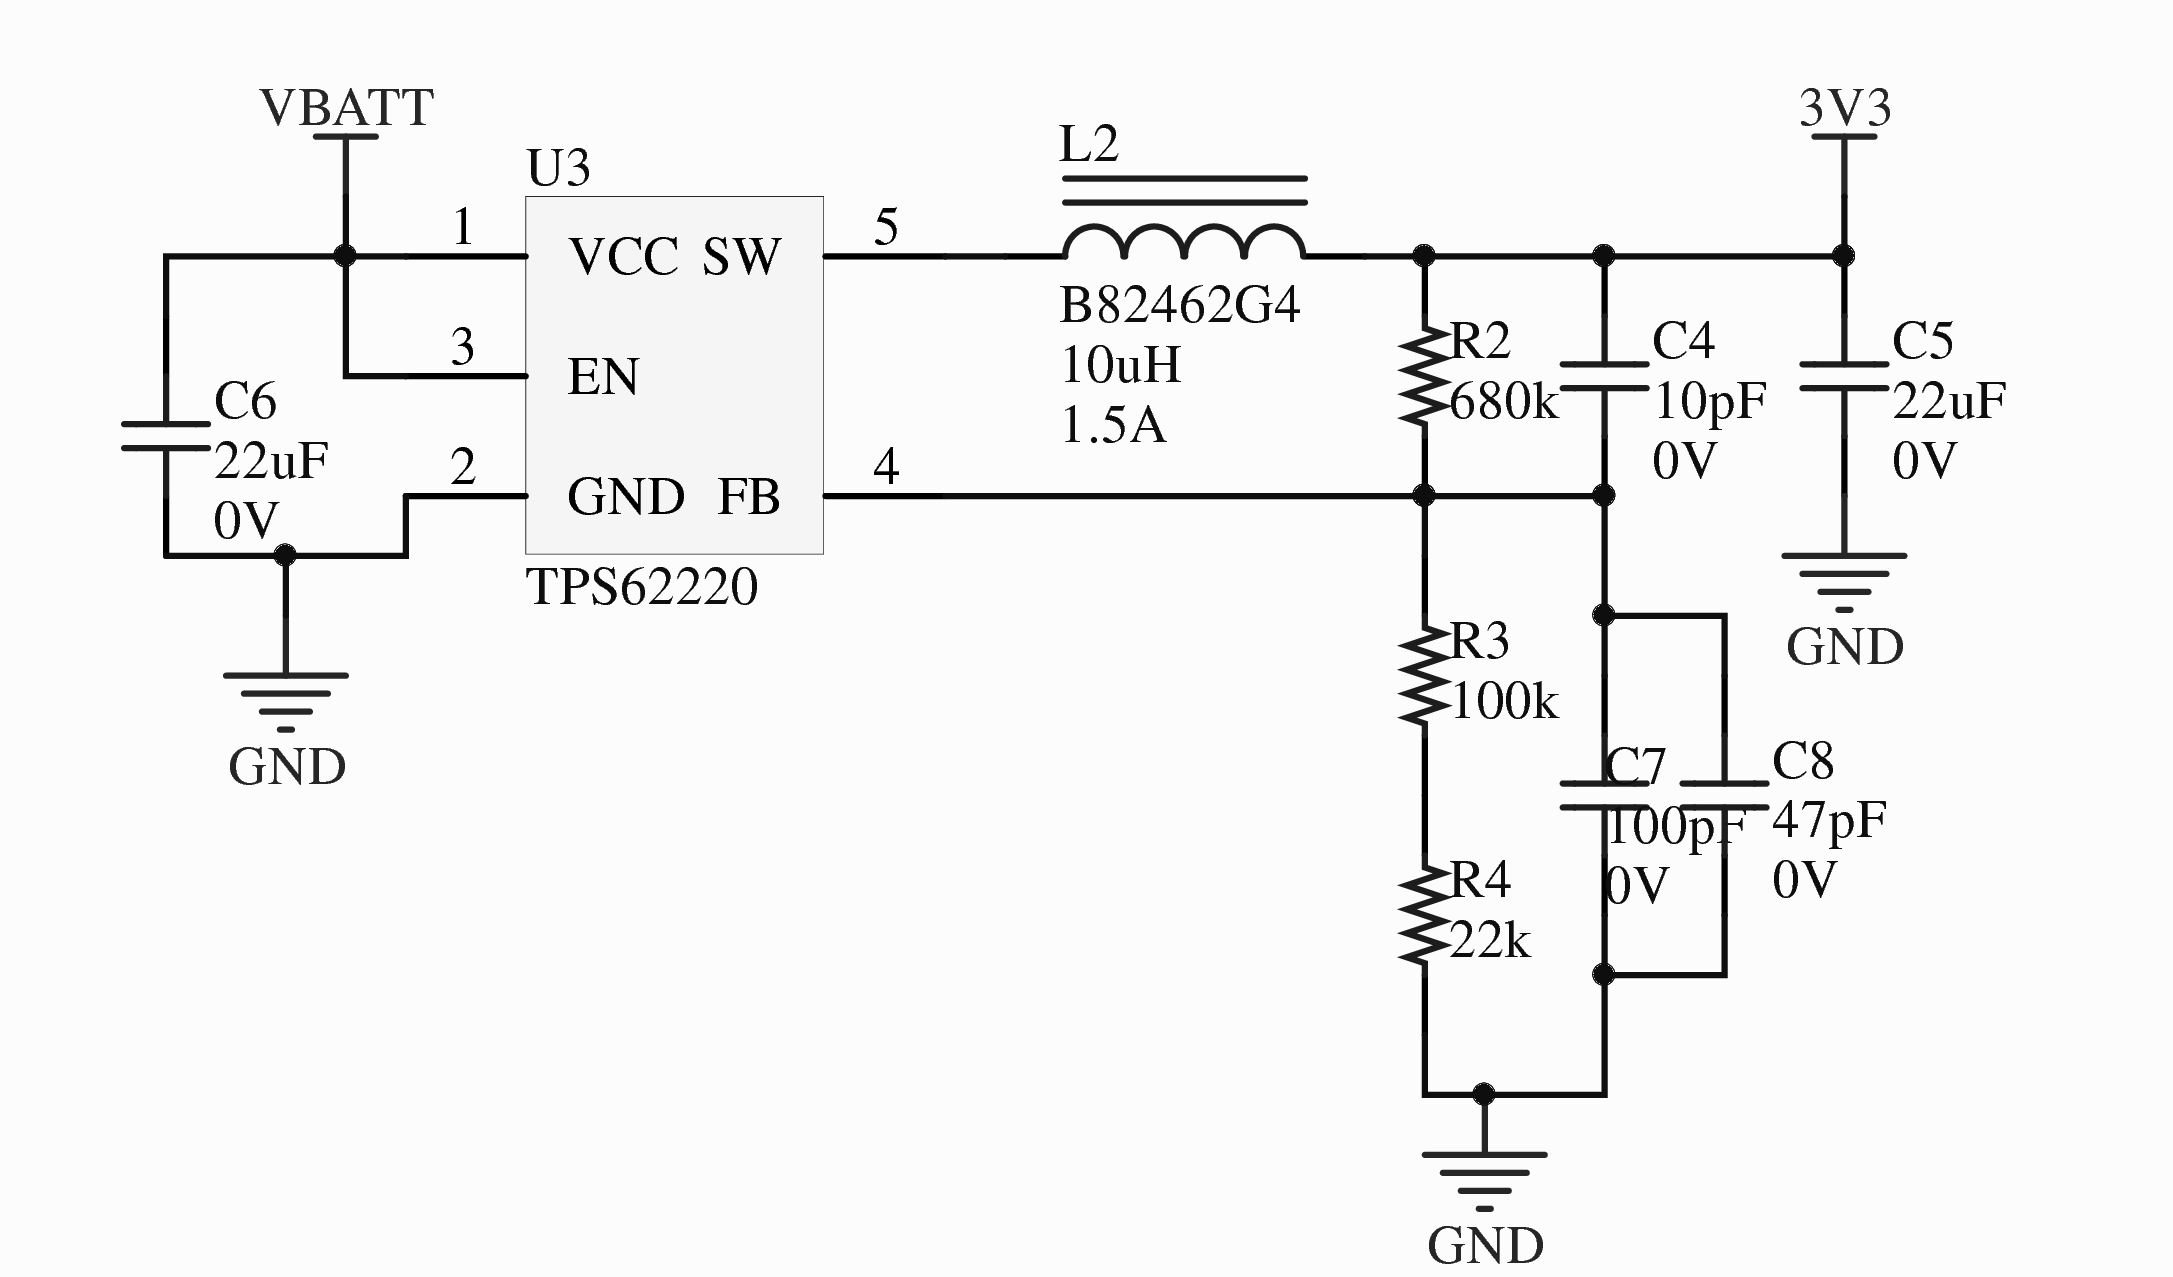
\includegraphics[width=.8\linewidth]{graphics/tps6220_circuit}
	\caption[3.3 V buck converter circuitry.]{Circuitry of Buck converter with an output voltage of 3.3V. \texttt{TPS62220} is used as the regulator.}
	\label{fig:tps62220_circuit}
\end{figure}
% subsection joint_design (end)

\subsubsection{Choosing a Battery} % (fold)
\label{ssub:choosing_a_battery}
\thomas{write few words on renata and difficulty of procurement (most capacity in 57mm and 9mm)}

\subsection{Joint Microcontroller}
\label{sub:joint_microcontroller}


\mikkel{Not finished}
\begin{itemize}
	\item Low power
	\item Compact size
	\item Three interrupt pins
	\item Eight I/O pins in total 
	\item SPI interface
	\item Non volatile memory
	\item 3.3V/5V supply
\end{itemize}


\begin{table}
	\centering
	\begin{tabular}{l}
		 \textbf{Requirements:} \\ \hline
		 Low power \\ \hline
		 Compact size \\ \hline
		 Three interrupt pins \\ \hline
		 Eight I/O pins in total\\ \hline
		 SPI interface \\ \hline
		 Non volatile memory \\ \hline
		 3.3V/5V supply \\ \hline
	\end{tabular}
	\caption{Hmmm. Not satisfied with this.}
	\label{tab:joint_mic_rec}
\end{table}

We chose the the ATtiny84 - yay!


\subsection{Voltage Rails}
\label{sub:voltage_rail}
It is necessary to determine which voltage rails are needed for the components on the joint board to function.
The wireless module, \texttt{NRF24}, and the ATtiny84 can both be run at 3.3V, but the Rolin encoder needs 5V.
Clearly a 3.3V rail and a 5V rail is needed. 
The current consumption on both rails need to be determined in order to specify the requirements for the voltage regulators and the required size of the battery needed.
\mikkel{There should be a nice introduction to this section about the Joint in general... Battery and so on.}


\paragraph{3.3V:}
\label{par:3_3v}
The \texttt{NRF24} module has maximum supply current of 12.3mA \cite{NFR24L01} and the \texttt{ATtiny82} has a maximum of 9mA \cite{attiny84}.
This totals 21.3mA of current that the 3.3V rail needs to supply.

\paragraph{5V:}
\label{par:5v}
The only component drawing current from the 5V rail is the Rolin encoder which has a maximum supply current of 20mA \cite{RLBD01}.

\subsection{Power Consumption} 
\label{subsub:power_consumption}
The power consumption at each rail is calculated and 

\begin{table}
	\centering
	\begin{tabular}{l|r|r}
		 Voltage rail 	& Current [mA] 	& Power [mW]\\
		 \hline
		 3.3V 			& 21.3			&70.3		\\
		 5V  			& 20 			&100		\\
		 \hline
		 Total 			& 				&170.3		
	\end{tabular}
	\caption{Power usage on voltage rails and in total.}
	\label{tab:power_joint}
\end{table}

\subsection{Battery}
\label{subsub:battery}
The physical dimensions of the battery is constrained by the free space in the designed joint.
It needs to be able to fit in a cylinder with a diameter of 57mm and height of 9mm.
Furthermore needs to have enough capacity to power the circuit for a full workday of a student, which is estimated to be 10 hours.
\mikkel{10 hours workday?}

\paragraph{9V Battery}
Batteries in the standard 9V package can purchased with with enough capacity, but the physical size disqualifies it.

\paragraph{Button Cell Battery}
Button cell batteries does live up to the physical constraints, but does not have the wanted capacity. 
Several of them can be put in series, but they still does not yield the wanted capacity.

\paragraph{Li-Ion Battery}
Lithium-Ion batteries have a very high energy density and it should therefore be possible to find a battery that fit both the physical and capacity constrains.
WE FOUND ONE!!!!!
3.7 Volt - YES!
3.7V to 4.2V - ca. =!=!??

\subsection{RS422}
No termination was used....
Under 200kbps....
Short wires...
minimum power.

See \cite{rs422_texas} page 13.

\subsection{Voltage Rail Generation}
\label{sub:voltage_rail_generation}
As described in section \ref{sub:voltage_rail}, a 5V and a 3.3V rail is needed. 

\subsubsection*{5V}
Generating 5V can be done by boosting the battery voltage up to 5V, as the battery voltage will always be lower than 5V.
The boost regulator \texttt{SP6641BEK-L-5-0} has an input range of 0.9V to 4.5V and an fixed output of 5V \cite{sp6641b}.
The circuitry used in this project will be based on the design of the boost converter explained in the datasheet.
\mikkel{Schematic of boost converter here?}

\subsubsection*{3.3V}
The task of generating 3.3V from the battery is complicated by the battery voltage varying from 4.2V down to 3.0V*.
\mikkel{Source needed when we know battery}

Three different solutions appeared after an initial analyse of the task:

\begin{itemize}
	\item Buck converter
	\item Buck-Boost converter
	\item Linear regulator
\end{itemize}

The qualities and drawbacks of the three solutions are presented here.

\paragraph{Buck Converter}
The voltage from the battery can be converted to 3.3V using a Buck converter.
A Buck converter is relatively simple and circuitry can easily be designed for the task.
It is only able to supply an output voltage that is lower than the input voltage.
Which means that when the battery voltage is lower than 3.3V the converter will stop producing a stable 3.3V output.
This means that a portion of the battery capacity cannot be used.
The \texttt{TPS62220} is a Buck regulator and generally has good specifications for this task. 
With an input voltage of 3.7V and an output voltage of 3.3V it has an efficiency of approximately 95\% with an output current in the range of 1mA to 20mA \cite{TPS6222}.
The minimum drop out voltage of the \texttt{TPS62220} is low, because it has a 100\% duty cycle mode.
In this mode, the the drop out voltage is purely defined by the \texttt{ON} resistance of the internal switch, the DC resistance of the external inductor and the output current.

The drop out voltage can be calculated using equation \ref{eq:drop_v_tps62}, \cite{TPS6222}.
\begin{equation}
	V_{drop} = I_{O} \cdot (R_{DS(on),max}+R_I)
	\label{eq:drop_v_tps62}
\end{equation}

\begin{equation}
	V_{drop} = 0.02 \cdot (0.67+0.09) = 15 [mV]
	\label{eq:drop_v_tps62_2}
\end{equation}

Where $I_O$ is the output current, $R_{DS(on),max}$ is the \texttt{ON} resistance of the internal switch and $R_I$ is the DC resistance of the external inductor.
The inductor resistance used is found in the \texttt{LQH55D} SMD inductor \cite{LQH55D}.
\mikkel{Update if new inductor is used}
This means that it can supply 3.3V output when the input voltage is 3.315V or greater



\paragraph{Buck-Boost Converter}
The motivation for using a Buck-Boost converter is to allow for full utilization of the battery capacity.
This requires that the converter can make a seamless transition between the stepping up and stepping down of the input voltage. 
\texttt{TPS6300} is a Buck-Boost regulator that has these features.
The external circuitry is simple, but the drawback of this regulator and converter is the efficiency of it.
With an input voltage of 3.7V and an output voltage of 3.3V it has an efficiency of approximately 75\% with an output current in the range of 1mA to 20mA \cite{TPS6300}.

\paragraph{Linear Regulator}
A linear regulator is a component that can regulate the output voltage by varying an internal resistance.
Linear regulators have a drop voltage that limit the output voltage. 
The \texttt{LD3985} has an ultra low drop voltage of 20mV at 50mA output current \cite{LD3985}.

Therefore the efficiency is proportional to ratio between the output and input voltage and can be estimated using equation \ref{eq:eff_lin} \cite{ap_note_140}.

\begin{equation}
	\eta \simeq \frac{V_{out}}{V_{in}}
	\label{eq:eff_lin}
\end{equation}

The battery voltage varies from 4.2?? to 3.3V, but the nominal voltage is 3.7V and this will be used as an estimate of the mean voltage of the battery.
Using this the mean efficiency can be estimated as shown in equation \ref{eq:eff_lin_val}.

\begin{equation}
	\eta \simeq \frac{3.3}{3.7} = 0.89 = 89\%
	\label{eq:eff_lin_val}
\end{equation}


\paragraph{Comparison}
The most important parameters of the three solutions discussed are shown in table \ref{tab:vol_gen_joint}.

\begin{table}[h]
	\centering
	\begin{tabular}{l|c|c|c}
		  				&	Buck 	& Buck-Boost 	& Linear\\
		 \hline
		 Efficiency  	&  95\% 	& 75\%			&89\%		\\
		 Drop out [mV]		&15  	& N/A		&20		\\
	\end{tabular}
	\caption[Parameters of voltage generation solutions.]{Parameters of the three solutions using a Buck converter, Buck-Boost converter or a linear regulator. The efficiency shown is estimated with an input voltage of 3.7V, an output voltage of 3.3V and an output current in the range of 1mA to 20mA. The drop out voltage is estimated with an output current of 20mA (Buck) and 50mA (linear regulator).}
	\label{tab:vol_gen_joint}
\end{table}

The Buck converter solution has the highest efficiency and is therefore the natural choice.
As already discussed the disadvantage of using a Buck converter is that the full battery capacity cannot be utilized.
A discharge test should be conducted to determine the amount of capacity that cannot be utilized.


\paragraph{Battery Discharge}
At the time of writing, the chosen battery has not yet been procured and the test will therefore be conducted on a similar battery instead.
The battery under test is a 850 mAH Li-Ion battery with the dimensions 49mm X 29mm X 6mm.
It should be noted that both the capacity and physical dimensions are similar to the chosen battery.
The discharge curve of the two batteries will not be identical, but will be sufficient close to to allow for deciding which solution should be used.
The test was conducted by connecting the battery to an electrical load programmed to discharge with a constant power of 0.3 Watt, while measuring the battery voltage.
The measured discharge curve is shown in figure \ref{fig:bat_discharge}.

\begin{figure}[h]
	\centering
    % This file was created by matlab2tikz.
%
%The latest updates can be retrieved from
%  http://www.mathworks.com/matlabcentral/fileexchange/22022-matlab2tikz-matlab2tikz
%where you can also make suggestions and rate matlab2tikz.
%
\definecolor{mycolor1}{rgb}{0.00000,0.44700,0.74100}%
%
\begin{tikzpicture}

\begin{axis}[%
width=4.521in,
height=3.566in,
at={(0.758in,0.481in)},
scale only axis,
xmin=0,
xmax=450,
xlabel style={font=\color{white!15!black}},
xlabel={Time [Min]},
ymin=2.5,
ymax=4.5,
ytick={2.5,   3, 3.5,   4, 4.5},
ylabel style={font=\color{white!15!black}},
ylabel={Voltage [V]},
axis background/.style={fill=white},
title style={font=\bfseries},
title={Discharge Curve of Li-Ion Battery}
]
\addplot [color=mycolor1, forget plot]
  table[row sep=crcr]{%
0	4.072\\
10	4.02699999999999\\
20	4.00799999999998\\
40	3.95999999999998\\
50	3.92200000000003\\
60	3.89499999999998\\
70	3.87900000000002\\
80	3.85500000000002\\
90	3.84300000000002\\
100	3.81799999999998\\
110	3.79700000000003\\
120	3.78899999999999\\
130	3.77699999999999\\
140	3.767\\
150	3.75299999999999\\
160	3.76100000000002\\
170	3.75999999999999\\
180	3.74000000000001\\
190	3.72500000000002\\
200	3.71300000000002\\
210	3.714\\
220	3.69999999999999\\
230	3.71100000000001\\
240	3.71199999999999\\
250	3.69999999999999\\
260	3.69299999999998\\
270	3.69099999999997\\
280	3.69799999999998\\
290	3.69099999999997\\
300	3.68099999999998\\
310	3.673\\
320	3.65699999999998\\
330	3.64499999999998\\
340	3.63499999999999\\
350	3.62299999999999\\
360	3.60700000000003\\
370	3.61399999999998\\
380	3.596\\
390	3.56799999999998\\
400	3.505\\
410	3.36099999999999\\
414.551694551695	2.30000000000001\\
};
\addplot [color=red, dashed, forget plot]
  table[row sep=crcr]{%
0	3.30000000000001\\
450	3.30000000000001\\
};
\end{axis}
\end{tikzpicture}%
	\caption{Voltages measured across a 850 mAH Li-Ion battery while discharging using an electrical load programmed to 0.3 Watt. Horizontal red line represents the 3.3V level.}
	\label{fig:bat_discharge}
\end{figure}
It can be observed that the battery voltage only drops below 3.3V for a very short time before the battery is completely discharged.

\paragraph{Conclusion}
The Buck converter solution has the highest efficiency and has a lower drop out voltage than the linear regulator solution.
The disadvantage of using a Buck converter is that the full battery capacity cannot be utilized, but a test showed that almost all of the capacity can be used.
Therefore it was chosen to use a Buck converter with the \texttt{TPS62220} regulator. 
The Buck converter circuit used is based on the recommendations in the datasheet of the \texttt{TPS62220}.
The circuit is shown in figure \ref{fig:tps62220_circuit}.

\begin{figure}[h]
	\centering
    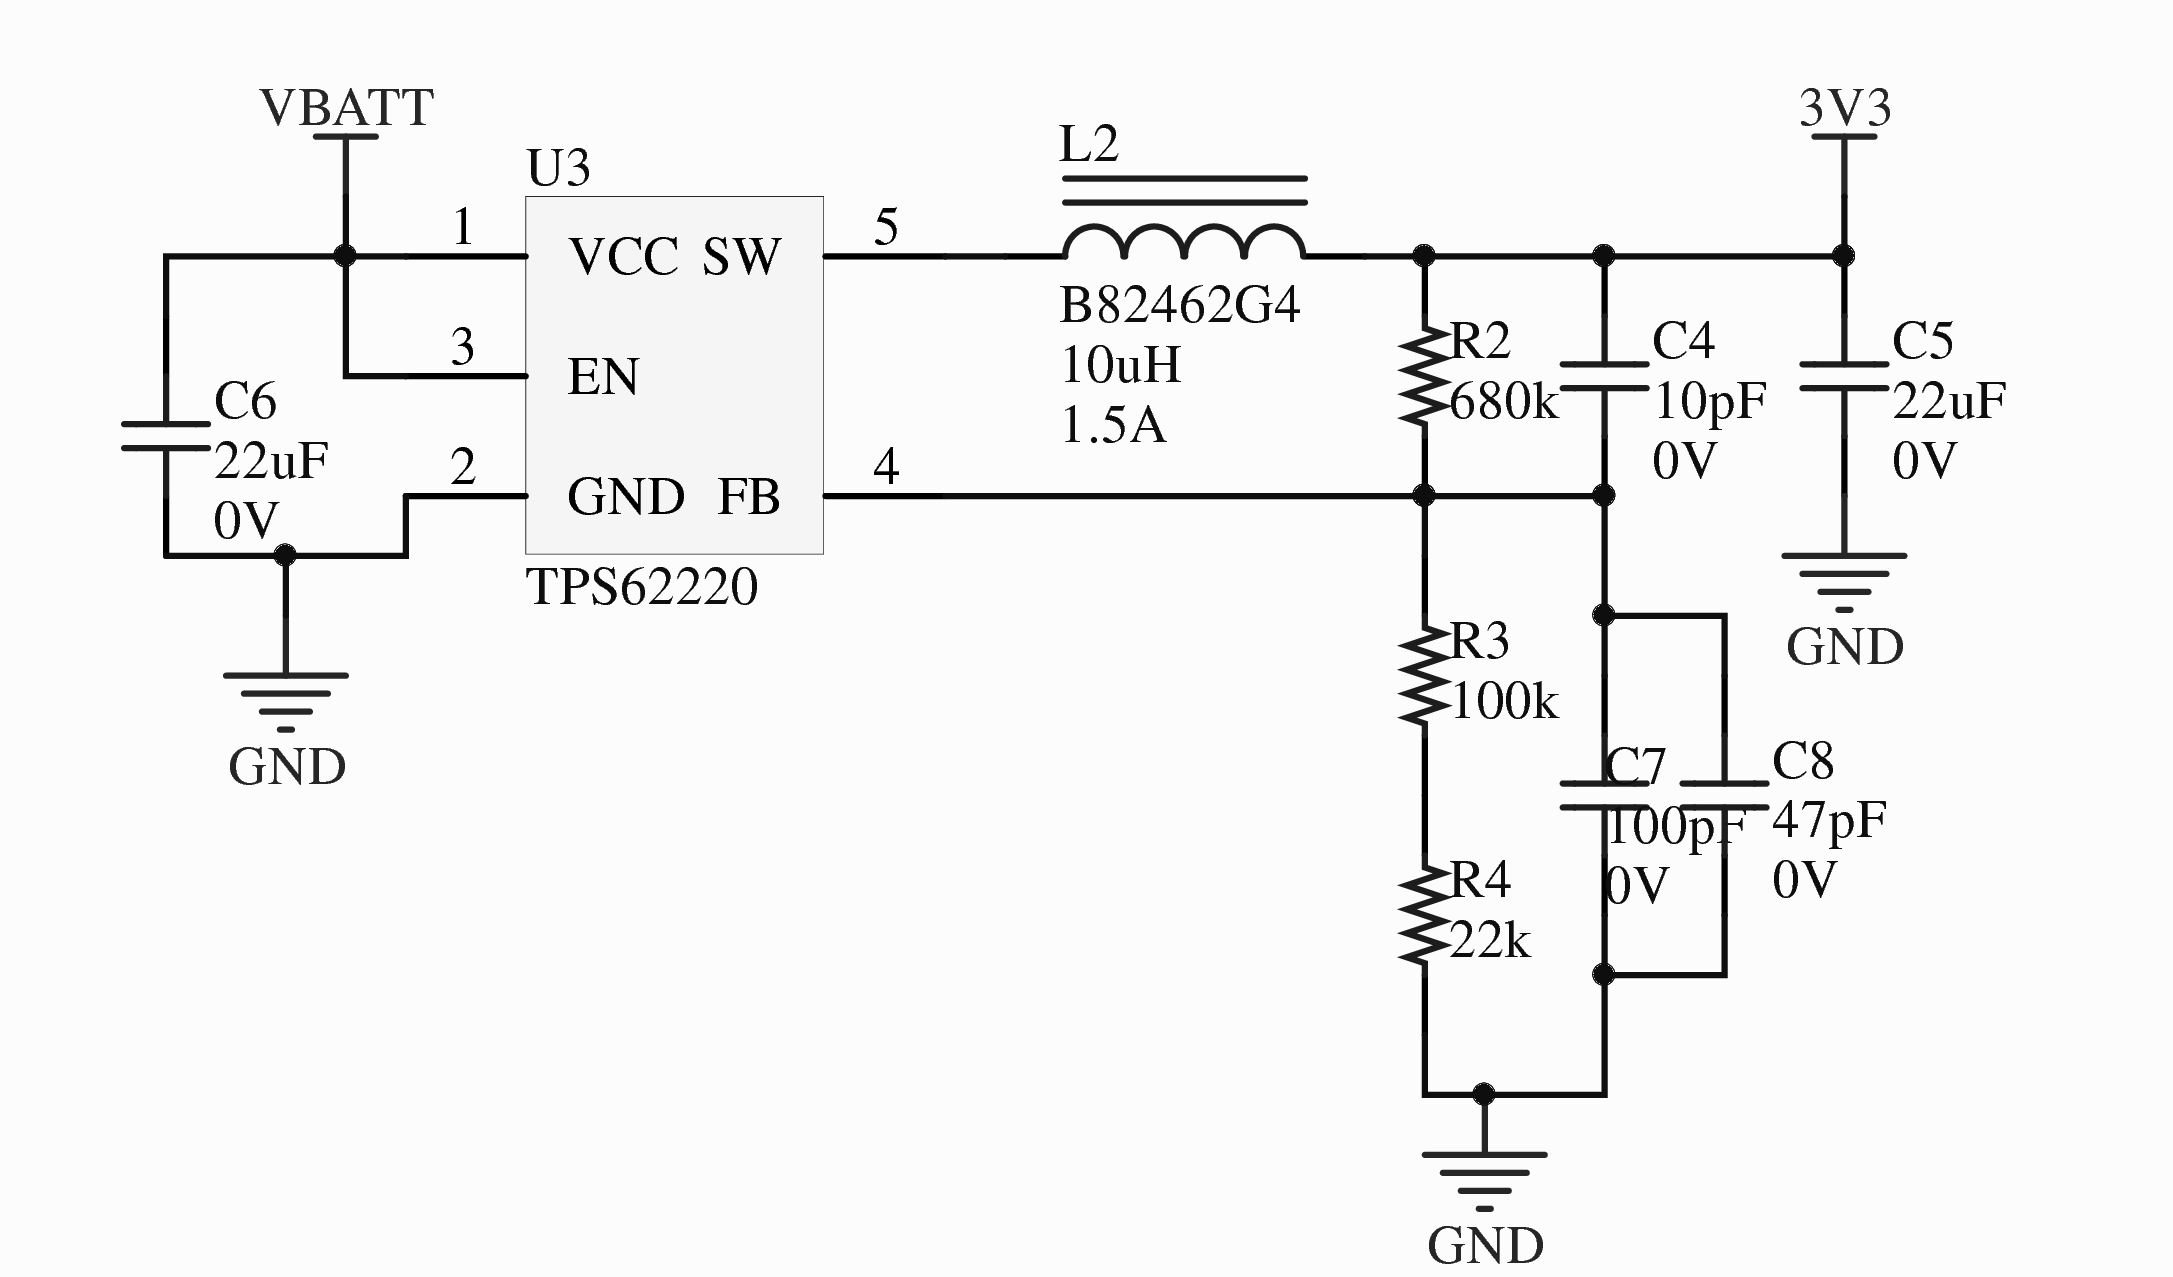
\includegraphics[width=.8\linewidth]{graphics/tps6220_circuit}
	\caption{Circuitry of Buck converter with an output voltage of 3.3V. \texttt{TPS62220} is used as the regulator.}
	\label{fig:tps62220_circuit}
\end{figure}
